\documentclass[12pt,a4paper]{article}
\usepackage{amsmath}
\usepackage{amsthm}
\usepackage{amsfonts}
\usepackage{amssymb}
\usepackage{amsmath,amscd}
\usepackage[symbol]{footmisc}
\usepackage{fancyhdr}
\usepackage{graphicx}
\usepackage{bm}
\usepackage[english]{babel}
\linespread{1.25}


\DeclareMathOperator{\Tr}{Tr}
\DeclareMathOperator{\D}{D}
\DeclareMathOperator{\Real}{Re}
\DeclareMathOperator{\T}{\text{\scriptsize T}}

\renewcommand{\thefootnote}{\fnsymbol{footnote}}


\begin{document}

\section{Hamiltonian Monte Carlo, code tests}

\begin{figure}[!htb]
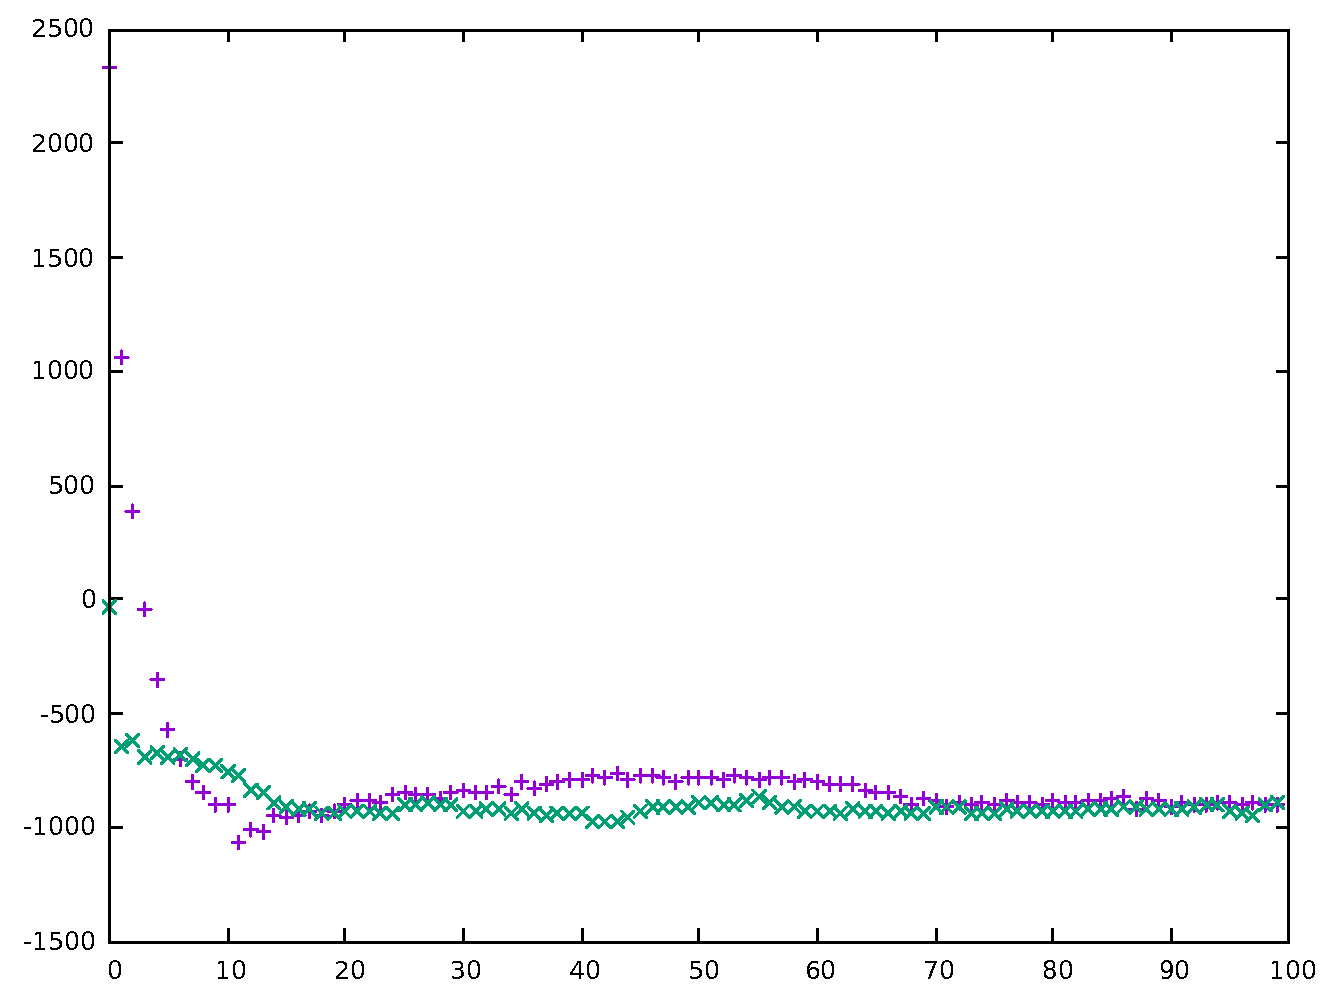
\includegraphics[width=1\linewidth]{p1q1n20g25.pdf}
\caption{Action $\Tr D^4 + g\Tr D^2$ vs Monte Carlo time; $(p,q)=(1,1)$; $n=20$; $g=-2.5$; $L=100$; $\tau_\text{cold10} = 0.0001$; $\tau_\text{cold90} = 0.0005$; $\tau_\text{hot} = 0.001$; time: 5s.}
\end{figure}

\begin{figure}[!htb]
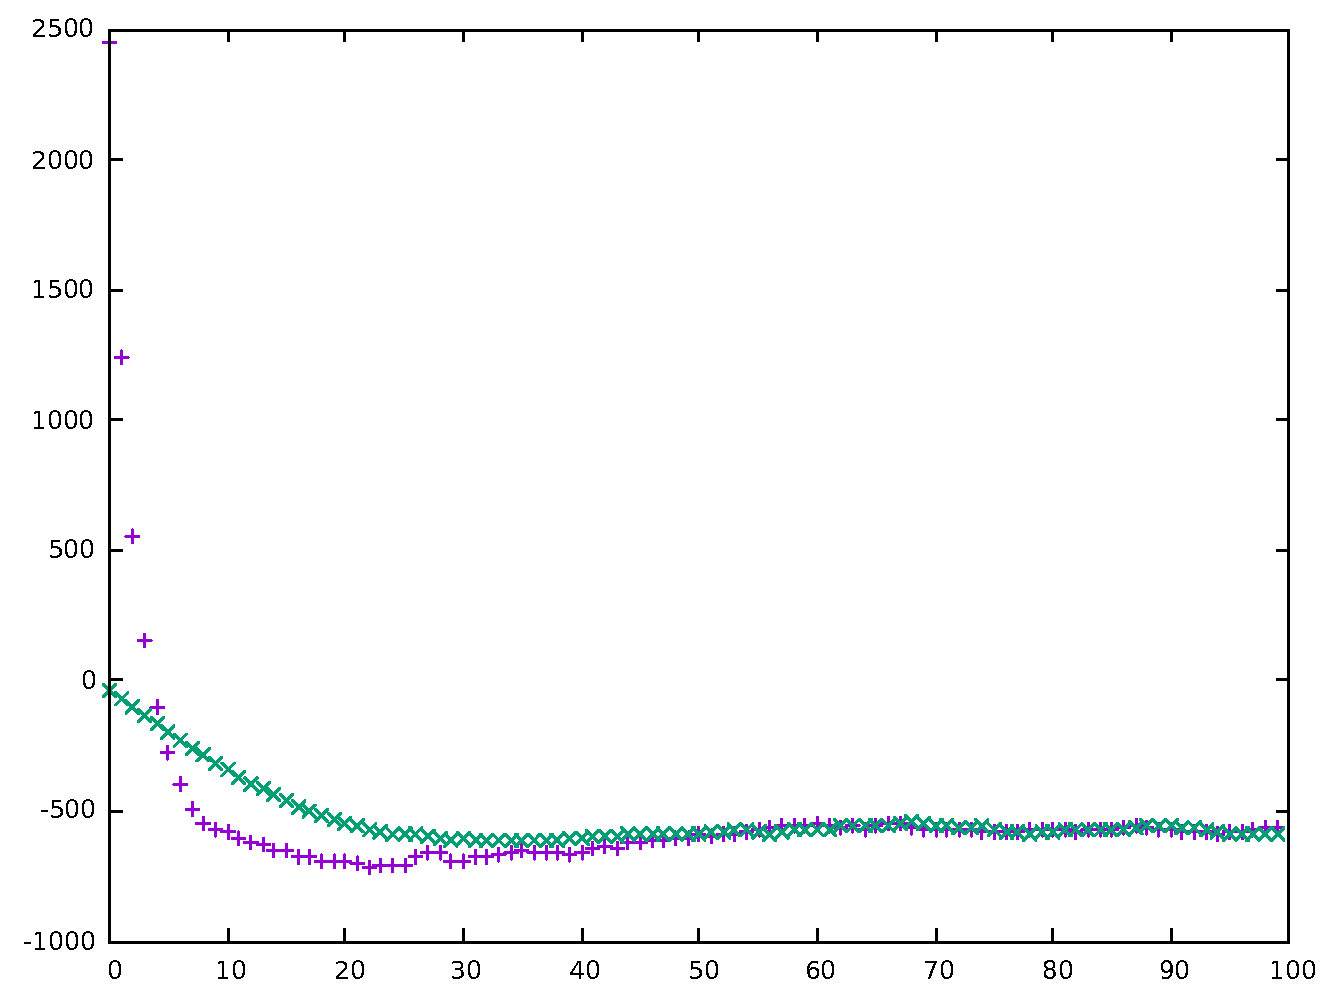
\includegraphics[width=1\linewidth]{p0q3n20g25.pdf}
\caption{Action $\Tr D^4 + g\Tr D^2$ vs Monte Carlo time; $(p,q)=(0,3)$; $n=20$; $g=-2.5$; $L=100$; $\tau = 0.0001$; time: 36s.}
\end{figure}

\begin{figure}[!htb]
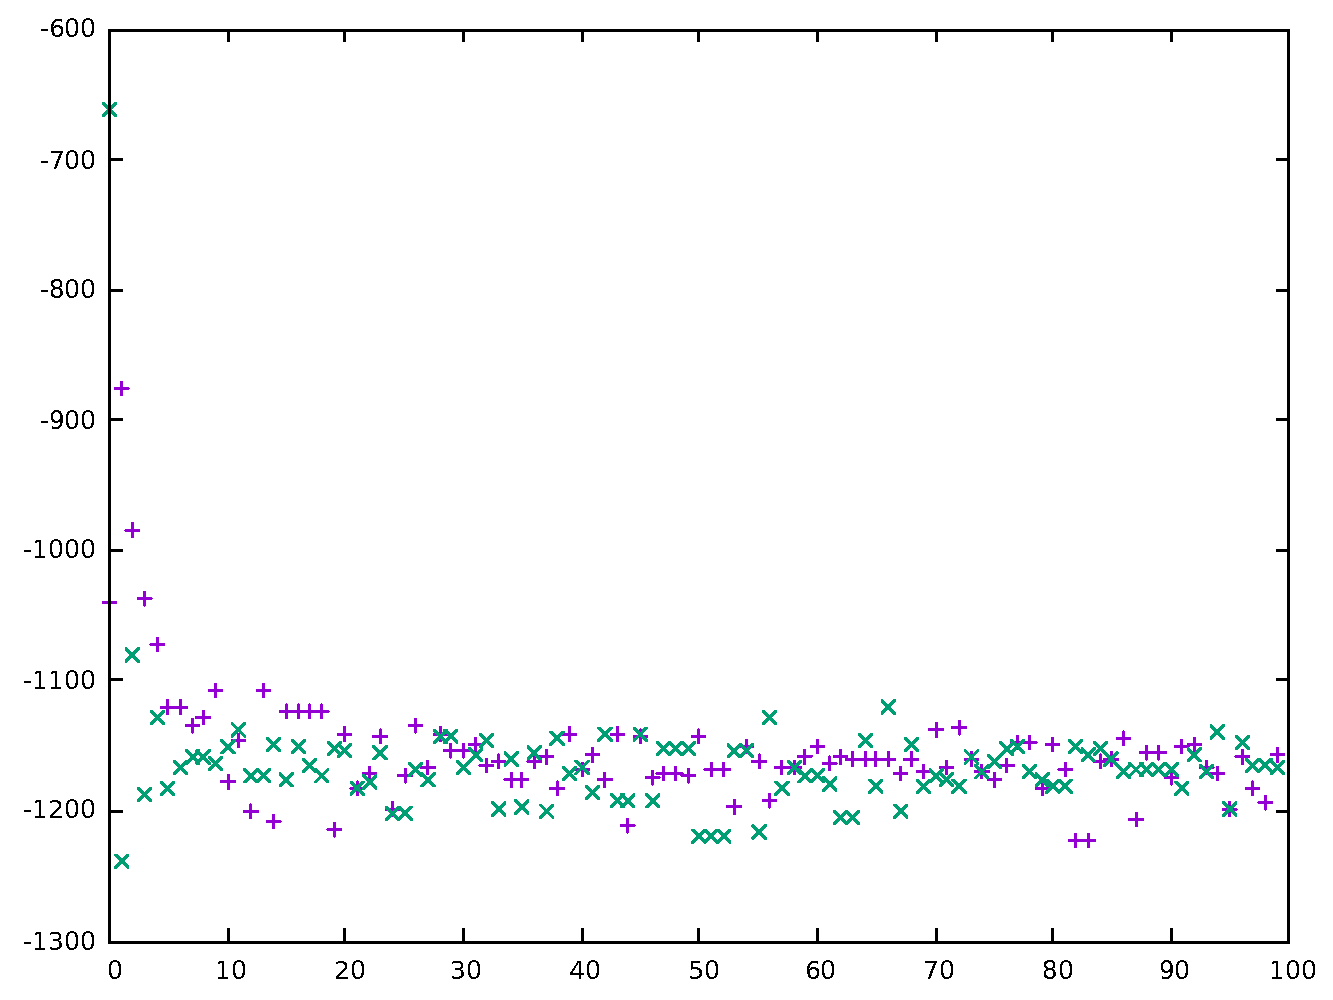
\includegraphics[width=1\linewidth]{p1q3n20g25.pdf}
\caption{Action $\Tr D^4 + g\Tr D^2$ vs Monte Carlo time; $(p,q)=(1,3)$; $n=20$; $g=-2.5$; $L=100$; $\tau_\text{cold10} = 0.001$; $\tau_\text{cold90} = 0.0005$; $\tau_\text{hot} = 0.0005$; time: 5m 40s.}
\end{figure}

\begin{figure}[!htb]
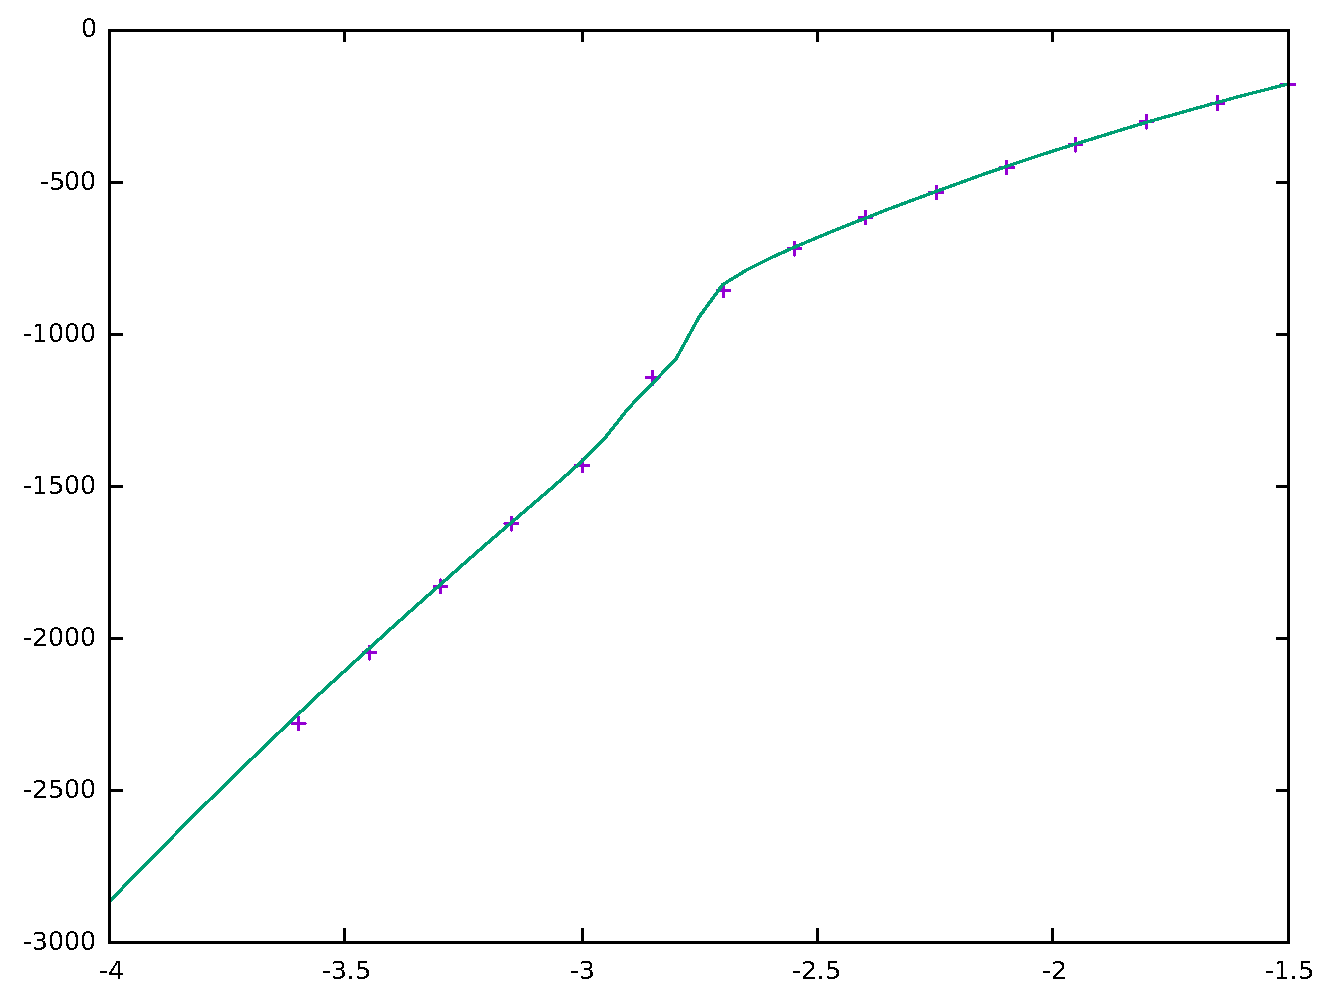
\includegraphics[width=1\linewidth]{p2q0n20S.pdf}
\caption{Action $\Tr D^4 + g\Tr D^2$ vs $g$; Metropolis (Green) and HMC (purple); $(p,q)=(2,0)$; $n=20$; $L=100$; $\tau = 0.0001$; time 13m 20s}
\end{figure}






\end{document}
